\subsection{Posterior Inference under the Extended Model}
\label{res:post_contour}
Figure~\ref{fig:contour} shows the joint posterior of $(\lambda, A)$ with the MAP estimate and HPD regions (39.3\% and 86.5\%). The MAP occurs at $\lambda \approx 0.0138$ and $A = y_{\max} \approx 179.45$ months, indicating that the estimate of $A$ coincides with the maximum observed tenure. This suggests that inference for $A$ is largely driven by the boundary condition $A \geq y_{\max}$ rather than information from the data.

The posterior of $\lambda$ is sharply concentrated, showing it is well identified, whereas $A$ remains highly uncertain. The HPD regions expand vertically along the $A$ axis and are truncated at the boundary, revealing that the uncertainty in $A$ mainly reflects “how much larger than $y_{\max}$” it could be. If the posterior were Gaussian and independent, the HPD bands would form concentric ellipses (See Figure~\ref{fig:hpd-example} in Section~\ref{sec: Contour Joint Posterior}); instead, the skewed shape highlights boundary-driven effects, while $\lambda$ is nearly independent of $A$.

This motivates the marginalization analysis in the next section, which checks whether integrating out $A$ preserves the inferential structure of $\lambda$ relative to the baseline exponential model.
\begin{figure}[H]
    \centering
    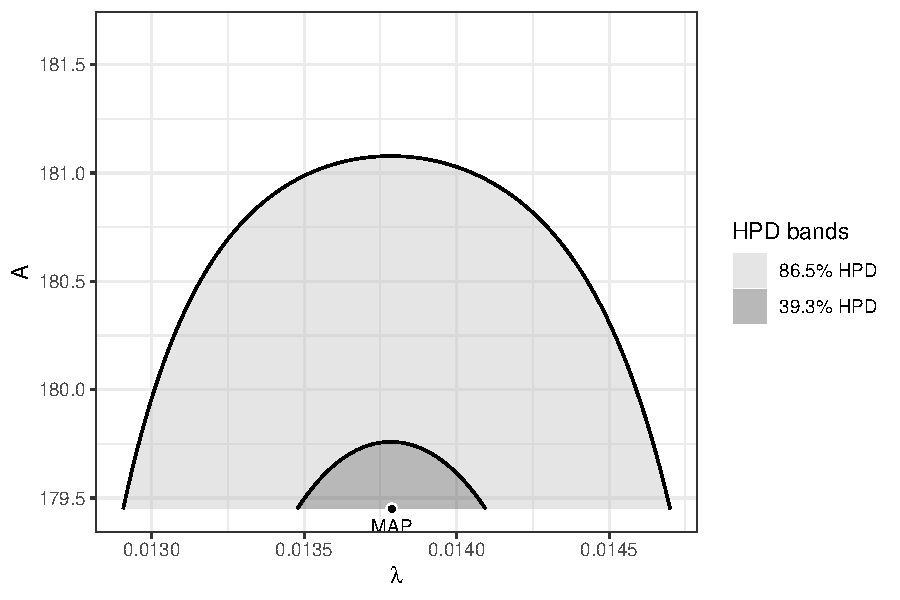
\includegraphics[height=9cm, width=0.65\textwidth]{images/post_contour.pdf}
    \caption{{\small Joint posterior $p(\lambda,A\mid\mathcal D)$ with 39.3\%/86.5\% HPD contours and MAP (black).}}
    \label{fig:contour}
\end{figure}


\subsection{Marginalization and Consistency Check}
\label{res:marginal}
Building on the boundary-driven geometry in Section~\ref{res:post_contour}, we now ask whether introducing $A$ changes inference on $\lambda$ once we focus on $\lambda$ alone. Figure~\ref{fig:marginal} compares the marginal posterior of $\lambda$ obtained from the extended model (blue; integrating out $A$ on the grid) with the analytic posterior from the baseline exponential model that does not include $A$ (red).

The two curves are visually indistinguishable across the entire support: the peak location, peak height, and tail decay coincide to plotting precision, and the associated credible intervals match to numerical accuracy. This confirms a key point for practice: Inference on $\lambda$ is preserved after introducing $A$. In the extended model, $A$ behaves as a (predictive) nuisance parameter: it is crucial for generating realistic fake data and for describing the observation window, but it does not alter the posterior for the event-time rate $\lambda$.

This empirical agreement is exactly what the factorization of the likelihood predicts (see Section~\ref{边际化章节}): the $\lambda$-dependent and $A$-dependent terms separate, so integrating over $A$ contributes only a normalizing constant that does not depend on $\lambda$. Consequently, the boundary-driven skewness seen along the $A$ direction in Section~\ref{res:post_contour} does not propagate into the marginal for $\lambda$.

\begin{figure}[H]
    \centering
    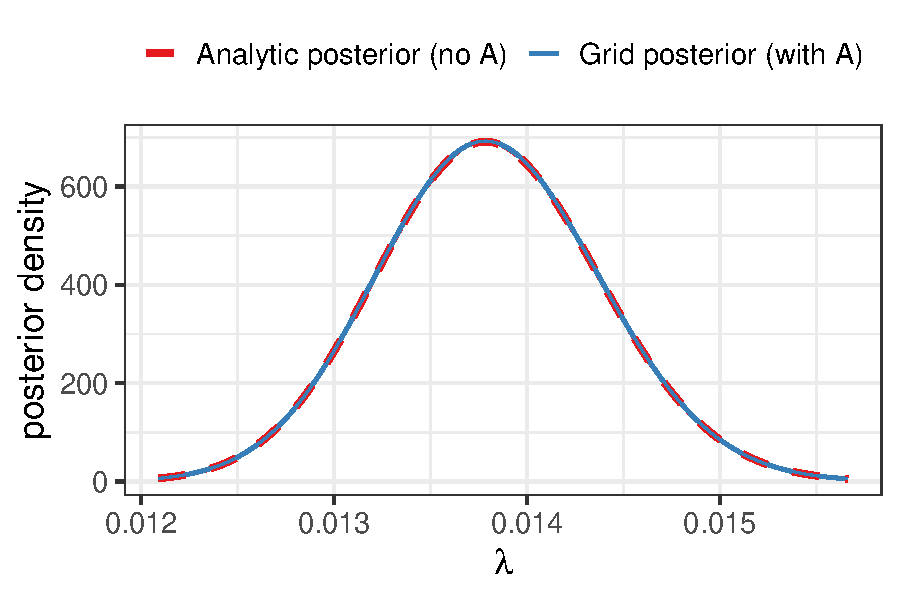
\includegraphics[height=6cm, width=0.7\textwidth]{images/lambda_marginal_compare.pdf}
    \caption{{\small Marginal posterior of $\lambda$ under the extended model (blue, obtained by integrating out $A$) versus the analytic posterior under the baseline exponential model (red).}}
    \label{fig:marginal}
\end{figure}
To further examine the stability of the marginal posterior for $\lambda$, we compared two sharply different priors for $A$: a weakly informative uniform prior $[y_{\max}, y_{\max}+500]$ and a truncated normal prior centered around $y_{\max}+50$. As shown in Figure~\ref{fig:diff_A_marginal}, despite the substantial difference in prior shapes, the resulting marginal posteriors for $\lambda$ are virtually identical.

This robustness is fully consistent with the theoretical result in equation~\eqref{eq:47} in Section~\ref{边际化章节}. As long as the prior for $A$ is independent of $\lambda$, integrating out $A$ contributes only a constant factor. Consequently, the marginal posterior of $\lambda$ is determined entirely by its likelihood and remains unaffected by the specific form of the prior on $A$.
\begin{figure}[H]
    \centering
    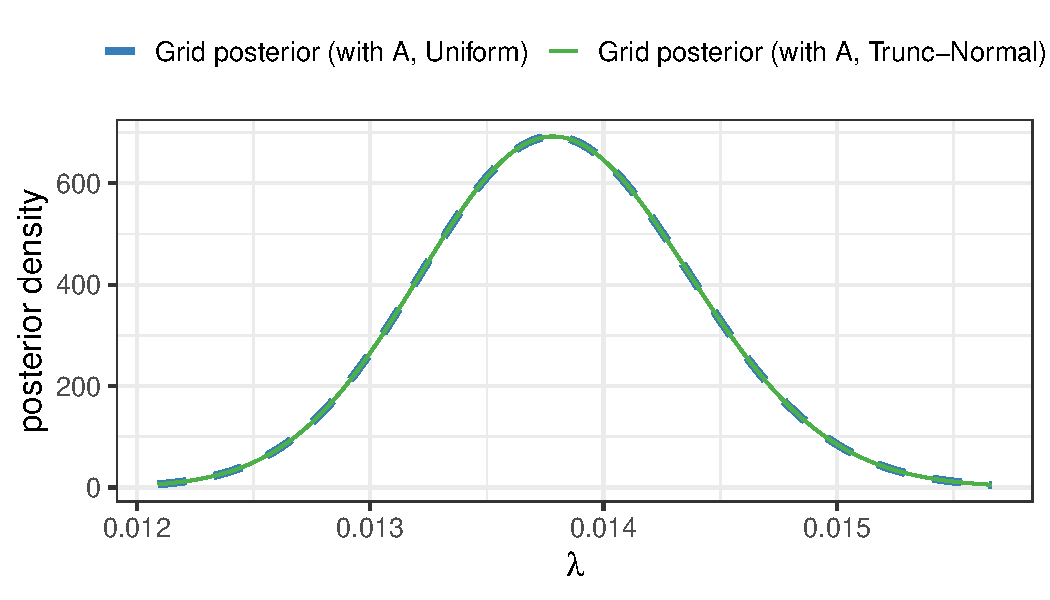
\includegraphics[height=6cm, width=0.75\textwidth]{images/diff_A_prior_marginal_compare.pdf}
    \caption{{\small Marginal posterior of $\lambda$ under two priors for $A$: uniform $[y_{\max}, y_{\max}+500]$ (blue) and truncated normal near $y_{\max}+50$ (green).}}
    \label{fig:diff_A_marginal}
\end{figure}
%%%%%%%%%%%%%%5
\subsection{Model checking}
\label{res: model checking}
\subsubsection{Simulation-based model checking}
While Section~\ref{res:marginal} showed that marginalizing out $A$ preserves the baseline inference on $\lambda$, such consistency does not guarantee that the baseline model itself adequately reflects the data. To further assess its validity, we first perform a simulation-based model check. Specifically, we generated pseudo-data with a fixed value $\lambda=0.05$ and refitted the exponential model. As shown in Table~\ref{tab:post-ci}, the posterior mean (0.053) and 95\% CrI [0.0496, 0.0567] successfully recover the true value, indicating that the model is structurally sound. For completeness, the full posterior histogram is provided in Supplementary Figure~\ref{fig:posterior_s1}.
\begin{table}[H]
\centering
\caption{{\small Posterior summaries and 95\% credible intervals (simulation-based model check)}}
\label{tab:post-ci}
\small
\begin{tabular}{lccccc}
\toprule
{Parameter} & {Mean} & {2.5\%} & {97.5\%} & {$n_{\text{eff}}$} & {Rhat} \\
\midrule
$\lambda$   & 0.0531 & 0.0496 & 0.0567 & 1113 & 1.000 \\
\bottomrule
\end{tabular}
\end{table}
%%%%%%%%%%
\subsubsection{Baseline Exponential Sensitivity to A}
\label{res:baseline_ecdf}
Having established that the baseline model is structurally coherent, we next examine its adequacy when applied to real data. As previewed in Section~\ref{Impact of A}, different choices of the observation-window parameter $A$ (e.g., 30, 200, 1000 months) lead to markedly different censoring patterns. Building on this, we now conduct posterior predictive model checking under the baseline specification, where the true value of $A$ is unknown. To generate the posterior predictive datasets, we draw the event-rate parameter at its posterior mean, $\hat{\lambda} \approx 0.0138$, and apply Algorithm 1 (Section~\ref{subsec:wo Layers of Model Checking}) with $n=1129$ simulated observations, matching the real sample size.

\textbf{Case $A=30$ (Figure~\ref{fig:ppc_a30}):} Predictive ECDFs for both events and censorings rise sharply at early times and diverge strongly from the observed curves. The nearly linear simulated curves approximate a uniform distribution, eliminating the exponential decay evident in the real data. This is reflected in Table~\ref {tab:modelcheck_counts} (events = 184 vs. 571 in real data; censored = 945 vs. 558), with censoring far too dominant. As shown previously in Figure~\ref{fig:fake-hist_a30}, durations are compressed into the 0–30 month range, meaning that a small $A$ forces most individuals into premature censoring and breaks the fit. \textbf{Case $A=1000$ (Figure~\ref{fig:ppc_a1000}):} The predictive ECDFs appear superficially closer to the observed curves, particularly in the tail, but this similarity is misleading. Under $A=1000$, censoring almost disappears (events = 1055, censored = 74), and the few censorings occur at implausibly long durations (see Figure~\ref{fig:fake-hist_a1000}), so the apparent fit is driven by a handful of late censoring points and fails to reproduce the roughly 50–50 balance of the real data. Moreover, a tenure length of 1000 months is itself unrealistic in any employment context.

In contrast, our \textbf{best-guess setting of $A=200$ (Figure~\ref{fig:ppc_a200})} yields results that are much closer to reality. For event times, the predictive ECDF follows the observed curve most closely, avoiding the steep rise under $A=30$ and the overly flat pattern under $A=1000$. For censored durations, the predictive ECDF is more reasonable than under either extreme, and the counts are far better aligned with the data (events = 752 vs. 571; censored = 377 vs. 558; see Table~\ref{tab:modelcheck_counts}), reflecting the censoring mechanism more faithfully, though events are still over-predicted and censoring under-represented.

While $A=200$ represents the most credible benchmark in terms of both curve shape and censoring balance, discrepancies in the ECDFs remain. This indicates that the survey window length directly affects our inference on tenure, motivating the extended Bayesian model with $A$ treated as a parameter.
\begin{figure}[H]
\centering
\begin{subfigure}[t]{0.8\textwidth}
  \centering
  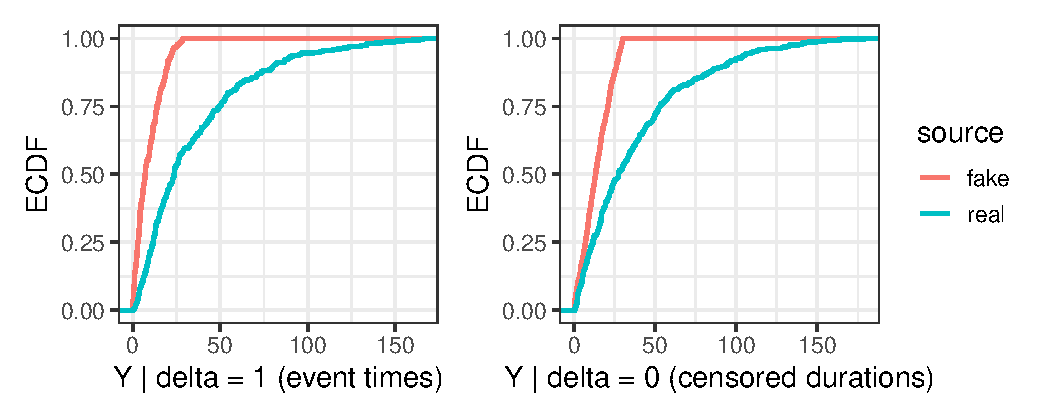
\includegraphics[height=4cm,width=\linewidth]{images/ppc_two_a30.pdf}   % 图3路径
  \caption{{\small $A=30$ months}}
  \label{fig:ppc_a30}
\end{subfigure}
\begin{subfigure}[t]{0.8\textwidth}
  \centering
  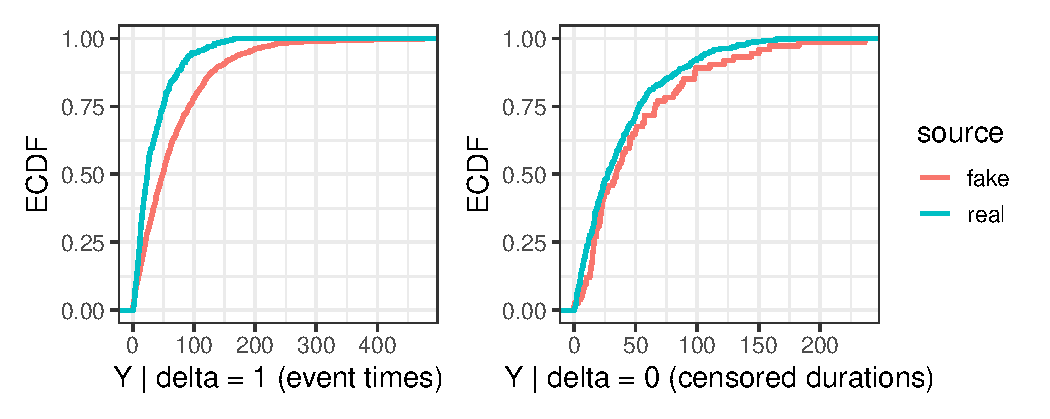
\includegraphics[height=4cm,width=\linewidth]{images/ppc_two_a1000.pdf}   % 图3路径
  \caption{{\small $A=1000$ months}}
  \label{fig:ppc_a1000}
\end{subfigure}
\begin{subfigure}[t]{0.8\textwidth}
  \centering
  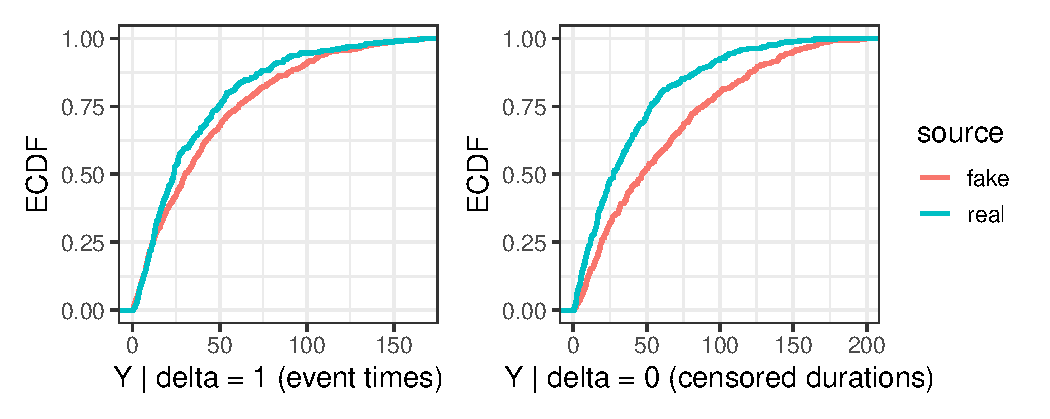
\includegraphics[height=4cm,width=\linewidth]{images/ppc_two_a200.pdf}   % 图3路径
  \caption{{\small $A=200$ months}}
  \label{fig:ppc_a200}
\end{subfigure}
\caption{{\small Posterior predictive ECDFs of event times (left) and censored durations (right) under different $A$.}}
\label{fig:ppc-A30}
\end{figure}
%%%%%%%%%%%
\begin{table}[H]
\centering
\caption{{\small Event and censoring counts in real and simulated datasets (model checking)}}
\label{tab:modelcheck_counts}
\small 
\scalebox{0.9}{
\begin{tabular}{lcc}
\toprule
\textbf{Dataset} & \textbf{Censoring ($0$)} & \textbf{Events ($1$)} \\
\midrule
Real data        & 558  & 571  \\
Simulated ($A=30$)   & 945  & 184  \\
Simulated ($A=200$)   & 377  & 752
\\
Simulated ($A=1000$) & 74   & 1055 \\
\bottomrule
\end{tabular}}
\end{table}
%%%%%%%%%%%%%%%%%%%%%%%%%%%
\subsubsection{Extended Exponential Reveals Persistent Mismatch}
Building on the above, we fit the extended model with $A$ treated as a free parameter. The joint posterior $p(\lambda, A\mid\mathcal D)$ yields MAP estimates $\lambda \approx 0.0138$ and $A \approx 179$ months. Using these MAP values in Algorithm 1, we generate posterior-predictive datasets; the resulting ECDFs are shown in Figure~\ref{fig:ppc_map}.
\begin{figure}[H]
    \centering
    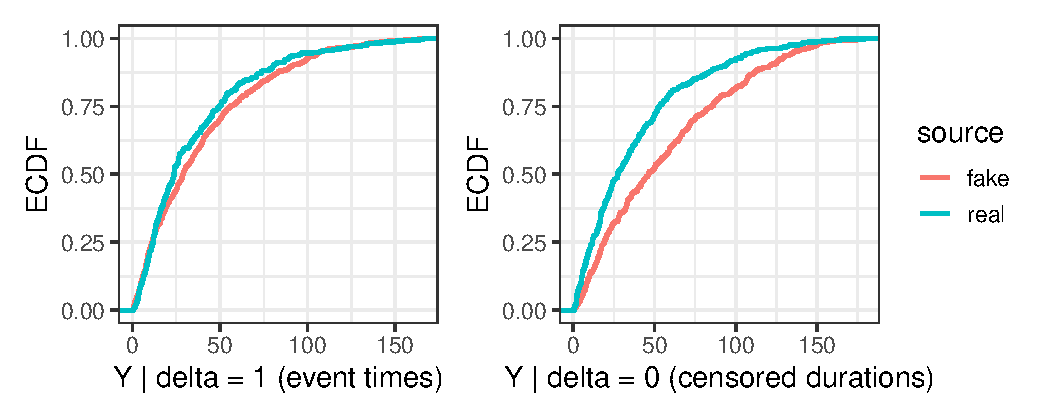
\includegraphics[height=4cm, width=0.8\textwidth]{images/ppc_two_map.pdf}
    \caption{{\small Posterior predictive ECDFs of event times (left) and censored durations (right) under the MAP estimates ($\lambda \approx 0.0138, A \approx 179$)}}
    \label{fig:ppc_map}
\end{figure}
Relative to the fixed-window benchmark $A=200$ (Figure~\ref{fig:ppc_a200}), the MAP setting produces a modest but consistent improvement: for event times, the gap to the observed ECDF narrows across 40–120 months, while for censored durations, the predictive curve shifts upward, reducing the under-representation of early censoring. Yet the discrepancies remain substantial. The model still underestimates censoring in the early months and over-smooths mid- to long-term durations, leaving systematic gaps in both panels.

This pattern is also reflected in the observed histograms (Figure~\ref{fig:离职数据分开的直方图}), which show a sharp early concentration of both events and censorings followed by a long, gradually declining tail. Such a shape implies a time-varying hazard, rising steeply at the start and decaying over time, whereas the exponential model enforces a constant hazard. The posterior-predictive checks, therefore, reveal that the mismatch cannot be fixed by tuning $A$ alone, but stems from the constant-rate assumption itself, motivating the exploration of more flexible duration models. A fuller discussion of these implications and possible alternatives is provided in Section~\ref{sec:discussion}.